\documentclass[9pt,conference]{IEEEtran}


\usepackage[utf8x]{inputenc}
\usepackage[magyar]{babel}
 %\usepackage{fontspec}
\usepackage{ucs}
\usepackage{amsmath}
\usepackage{amssymb}
\usepackage{graphicx}
\usepackage{amsfonts}
\usepackage{textcomp}

\usepackage{multirow}

 \usepackage{psfrag}
 \usepackage{subfig}
 
\usepackage[T1]{fontenc}

\begin{document}

	\title{Elektrosztatikus mérés szimulációja multiprocesszoros környezetben}
	
	\author{
		\IEEEauthorblockN{Bakró-Nagy~István} \IEEEauthorblockA{ Szélessávú
		Hírközlés és Villamosságtan Tanszék\\ Budapesti Műszaki és Gazdaságtudományi
		Egyetem \\ Budapest \\ \texttt{bakro.istvan@gmail.com}} 
		\and
		\IEEEauthorblockN{Reichardt András} \IEEEauthorblockA{Szélessávú Hírközlés és
		Villamosságtan Tanszék\\ Budapesti Műszaki és Gazdaságtudományi Egyetem \\
		Budapest \\ \texttt{reich@evt.bme.hu}}
	}
	
	\maketitle

	\begin{abstract}
	 Fémezett, töltött felület felett lévő fémtűre ható erő számítását végeztük el.
	 A szimulációk során a lehetséges párhuzamosításokat felhasználva a számítási időt csökkentettük.
	 Kidolgoztunk egy egyszerű szimulációs keretrendszert a felületmérés pontatlanságainak kiegyensúlyozására, az elérhető felbontás javítására.
	\end{abstract}

	\begin{IEEEkeywords}
	 numerikus szimuláció, parallel computing,\\ OpenCL, AFM 
	\end{IEEEkeywords}

	
	% Motivacio, Leiras

 
 \section{Motiváció} 
 
	Korábban elvégzett atomerő mikroszkópos mérések (AFM) validálása során az
	alábbi probléma keletkezett.
	A fémezett felület topológiáját mérések eredményeként ismerjük adott
	pontossággal.
	A mérések egy négyzetes háló felett történtek, amelynek mindkét irányban ($xy$)
	azonos felbontása volt.
	A mérés során a fémezett felülettől mindig azonos távolságra lévő, hosszú hegyes tűre ható erőt mértük,
	amikor a felület és a tű között adott, állandó feszültséget kapcsoltunk.
	
	A tűre ható erőt mérve a felület tű alatti tartományban található töltéseloszlásról kapunk információt.
	Végső cél olyan szimulátor építése, amelynek segítségével közel valós időben 
	lehetséges felületmérés alapján a felületli töltéseloszlásról információt
	kapni.
	
	A cikkben felhasznált mérési eredmény (\ref{fig:felulet}. ábra) egy
	$512\times512$ méretű tömb, amely értékei $0-255$-ig terjed.
	
	\begin{figure}[!h]
		\centering
		\includegraphics[width=0.45\columnwidth]{kepek/afm200.eps}
		\includegraphics[width=0.45\columnwidth]{kepek/efm200.eps}
		\caption{Méréssel kapott felület (balra) és szimulációval kapott töltéstérkép}
		\label{fig:felulet}
	\end{figure}
	
	
	
	\section{Szimuláció} 
	
	\subsection{Fizikai probléma leírása} 
	
	A megoldandó feladat egy elektrosztatikus feladat.
	A  határfeltételek a felület fémezése, amely zérus potenciálú és az adott
	potenciálú ($U_{pot}$) tű fémes felülete.
	A határok többi részén homogén Neumann feltételt alkalmazhatunk a szimmetriák és a töltésmentesség miatt.
	
	A belső térben nincsenek töltések, így itt a Laplace-egyenlet érvényes
	\eqref{eq:1}.
	
	\begin{equation}\label{eq:1}
		\Delta \ U(x,y,z) = 0 
	\end{equation}
	
	Ennek megoldására lehetséges direkt és iteratív megoldó algoritmusokat alkalmazni.
	Mindkét módszer esetében a 3 dimenziós probléma esetében téren diszkretizáljuk a problémát,
	amelynek vízszintes felbontása $\Delta_x$ és $\Delta_y$, míg függőlegesen $\Delta_z$.
	Az így kapott térbeli háló minden pontjához hozzárendeljük az $U_{i,j,k}$ potenciált
	 ($1\leq i\leq i_{max}$, $1\leq j\leq j_{max}$, $1\leq k\leq k_{max}$). 
	
% 	Az alkalmazott interpoláció során a függőleges irányú felbontást is figyelembe véve 
	A párhuzamosítási szándékok miatt az iteratív megoldást választottuk.
	Ekkor nem teljesen pontos megoldást kapunk, azonban kevesebb lépéssel
	juthatunk el a kívánt eredményhez.
	A számítási pontosság növelhető keményebb konvergenci követelmény
	megszabásával, ami további iterációkat jelent.
	
	Az iteratív megoldás során a megoldás aktuális értékének kiszámításához az
	előző megoldásból indulunk ki.
	A \eqref{eq:2} alapján végezzük az iterációt.
		\begin{multline} \label{eq:2} 
			U_{ijk}^{n+1} = \\ \Delta_1 \cdot \left(U_{i-1,j,k}^n+U_{i+1,j,k}^n
			+U_{i,j-1,k}^n+U_{i,j+1,k}^n\right)+ \\
							\Delta_2 \cdot \left(U_{i,j,k-1}^n+U_{i,j,k+1}^n\right)
		\end{multline}
	ahol $U_{i,j,k}^n$ az az $n$-dik iterációs lépésben az $i,j,k$ koordinátájú
	pontban mérhető potenciált jelöli, $\Delta_1$ a vízszintes felbontásból,
	$\Delta_2$ a függőleges felbontásból adódó állandó.
	Az iterációs eljárás előnye, hogy implementációja egyszerűbb és a
	\eqref{eq:2} szerinti ``simítás'' gyorsabb, mint a direkt megoldás.
	%Az iterációs eljárás előnye, hogy memóriaigénye kicsi a direkt megoldás során
	% adódó egyenletmegoldáshoz képest.
	%Hátránya hogy nem ad pontos választ egy lépésben.
	
	\begin{figure}[!ht]
		\centering
		\psfrag{ijk}{$(i,j,k)$}
		\psfrag{imjk}{$(i-1,j,k)$} 
		\psfrag{ipjk}{$(i+1,j,k)$}
		\psfrag{ijmk}{$(i,j-1,k)$} 
		\psfrag{ijpk}{$(i,j+1,k)$}
		\psfrag{d1}{$k_x$} 
		\psfrag{d2}{$k_y$} 
		\psfrag{d3}{$k_z$} 
		\psfrag{ijkm}{$(i,j,k-1)$} 
		\psfrag{ijkp}{$(i,j,k+1)$} 
		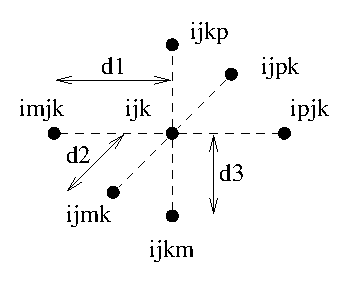
\includegraphics[width=0.95\columnwidth]{kepek/sema.eps}
		\caption{Diszkretizálás során alkalmazott felosztás} 
	\end{figure}

	
% 	fi(idx,idy,idz) = KK1*(fip(idx-1,idy,idz)+fip(idx+1,idy,idz)+fip(idx,idy-1,idz)+fip(idx,idy+1,idz))+...
%               KK2*(fip(idx,idy,idz-1)+fip(idx,idy,idz+1))

	\subsection{Szimuláció felépítése} 
	
	Mivel a Coulomb-kölcsönhatás a távolság négyzetével fordítottan arányos,
	így egy pont szomszédjait, pontosabban egy redukált környezetét szükséges
	csupán szimulálni.
	Ezzel az elhanyagolással már numerikusan kezelhető bonyulultságú problémára
	jutunk.
	
	Ezen módon egy mért pont $3\times3$-as környezetét vesszük figyelembe,
	a középső pont felett lévő felső elektródát feltételezve.
	A szimulációs felületen belül a mért magassági értékeket
	mint mintákat 2D-ben interpoláljuk.

	A szimulációk során a felület magasságának mérési adatait már ismertnek feltételezzük.
	A teljes mérőfelület pontjait külön-külön vizsgáljuk.
	Egyetlen pontban a mérési eredmény kiszámításának lépései az alábbiak :
	
	\begin{enumerate}
		\item A pont körüli felület $3\times3$-as mérési részének megállapítása,
		\item Közbenső (virtuális) mérési pontokkal a belső felbontás növelése
		interpolációval,
		\item Szimulálandó tér méretének számítása,
		\item Direkt/iteratív megoldó algoritmussal a tér meghatározása, 
				a tűre ható erő számítása illetve a tű alatti töltésmennyiség számítása,
		\item Adatok mentése.
	\end{enumerate}
	


	

	
	 \section{A szimulátor bemutatása} 
 A prototípus algoritmus fejlesztése MATLAB környezetben történt, ami később
 referenciaként szolgál.
 Alap MATLAB utasításokat használva több órát vesz igénybe a szimuláció
 futtatása.
 A MATLAB Parallel Toolbox-nak segítségével a szimulációt lehetséges
 párhuzamosan több processzormagon futtatni. Ezzel párszoros sebesség
 növekezés érhető el.
 A következőkben magát az algoritmust és az OpenCL keretrendszerben történő
 implementációját mutatjuk be.
 Majd az eredmények bemutatása során kerül összevetésre kerül a MATLAB
 referencia, a MATLAB Parallel Toolbox segítséggel, az OpenCL processzoron és
 az OpenCL GPU-n való futtatási ideje.
	
	\subsection{A lépések részletezése} 
		\subsubsection{Interpoláció}
		A korábban elmondottak alapján a felületet további mérési pontokkal egészítjük ki.
		Az extra mérési pontokat a legegyszerűbb síklapos közelítéssel alkothatjuk meg,
		a magasságmérési felbontás figyelembevételével.
		A szimulátorban egy általánosabb módszert alkalmazunk,
		ami egy 2D-s mozgó átlagoló szűrővel való simítás.
		A szűrővel aluláteresztést tudunk elérni, ami a minta magasságának
		mintavételezése utáni rekonstrukcióját jelenti. Egy ilyen interpoláció
		eredményét láthatjuk a \ref{fig:33pont}. ábrán. 
		
		\begin{figure}[!ht]
			\centering
			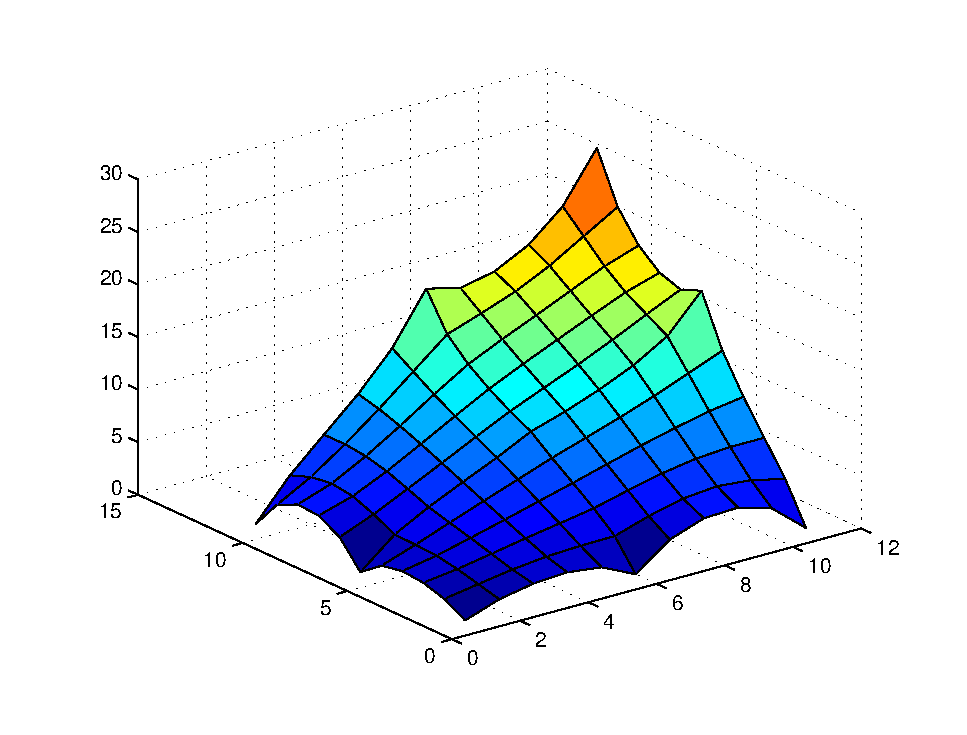
\includegraphics[width=0.95\columnwidth]{kepek/3x3_interpol.eps}
			\caption{$3\times3$ mérési pont $11\times11$ pontba való interpolációja}
			\label{fig:33pont}
		\end{figure}
		
		\subsubsection{A szimulálandó tér mérete}
		A szimulálandó tér (hasáb) magasságát a következő két mennyiség közül a
		nagyobbikkal határoztuk meg:
		\begin{itemize}
			\item Középső pont fölött lévő tű közepének magassága,
			\item A ($3\times3$) környezet legalacsonyabb és legmagasabb pontjának
			különbsége.
		\end{itemize}
		
		\begin{figure}[!h]
			\centering
			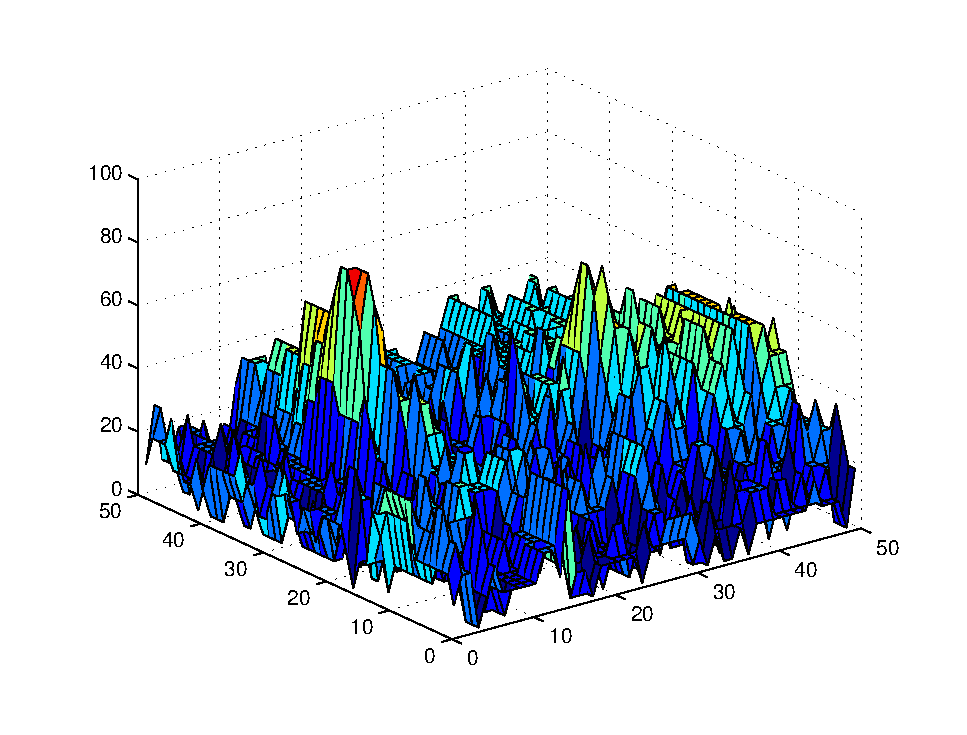
\includegraphics[width=0.45\columnwidth]{kepek/dimage.eps}
			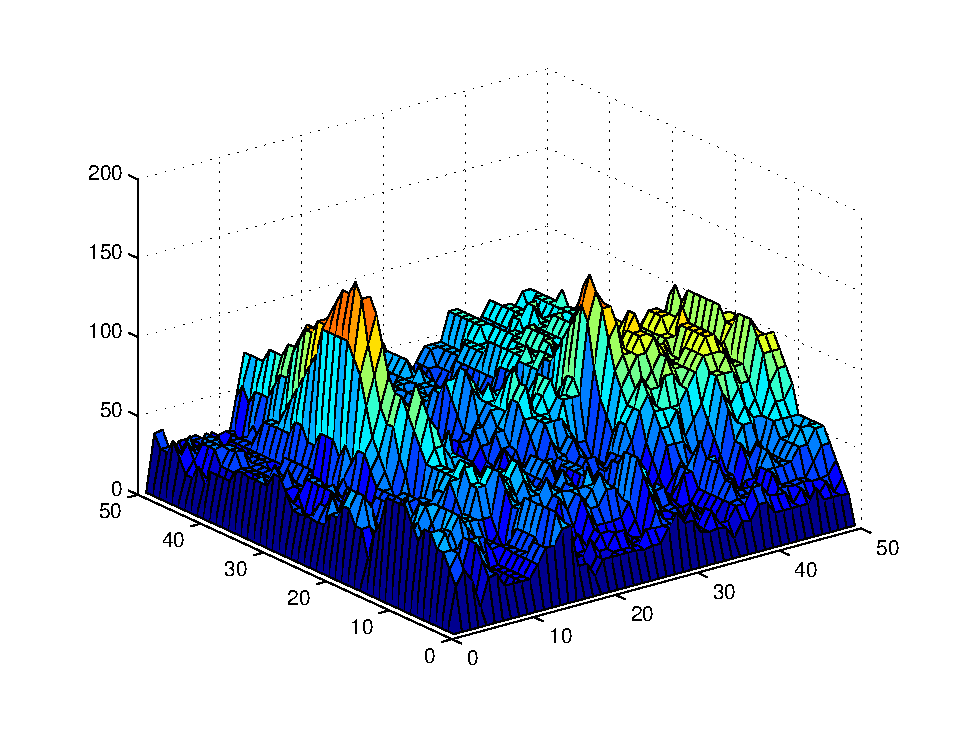
\includegraphics[width=0.45\columnwidth]{kepek/numh.eps}
			\caption{A magasságmérés eredményének részlete (balra) és a hozzá tartozó
			szimulálandó tér magassága.}
		\end{figure}
		
		\subsubsection{Iteratív megoldó algoritmus}
		Az iterációhoz a térháló pontjaihoz két mátrixot (tömbböt) rendelünk, ami a
		pontok potenciáljának aktuális ($\mathbf{U_{now}}$) és előző ($\mathbf{U_{prev}}$)
		értékeit tartalmazza.
		Az aktuális értékeket \eqref{eq:2} szerint számítjuk, majd az egész térre
		számítjuk az előzővel vett különbségének négyzetösszegét (normáját). E mérték
		képviseli a konvergencia szintjét, amit az iteráció során vizsgálva jutunk el a
		kívánt konvergencia szintre.
		Ha nem értük el a konvergencia szintet, akkor az előző két mátrixot
		felcserélve iterálunk tovább.
		
		\subsubsection{Adatok mentése}
		Tesztelhetőségi megfontolások végett a nem csak a tűre ható erőt (villamos
		térerősséget) exportáljuk, hanem a konvergencia szintjének változását és az
		interpolált felületet is. Az exportálandó menyiségek könnyen kézben tartható
		mérete miatt egyszerű CSV fájlként kerülnek mentésre. Ezen fájlok további
		poszt-processzálása MATLAB avagy munkalap kezelő szoftverrel is elvégezhető.
		
	
	\subsection{OpenCL architektúrája}
		Az Open Computing Language (OpenCL) keretrendszer \cite{opencl} közös
		nyelvet, magas szintű programozási interfészt és hardware absztrakciót nyújt a fejlesztőknek
		adat- vagy feladat párhuzamos számítások gyorsítására különböző
		számítóegységen (CPU, GPU, FPGA, DSP, \ldots).
		Az OpenCL modellje a különböző ``device''-okat, amik több ``compute unit''-ot
		(processzor-magot) tartalmaznak heterogén módon kezeli. 
		
		\begin{figure}[!ht]
			\centering
			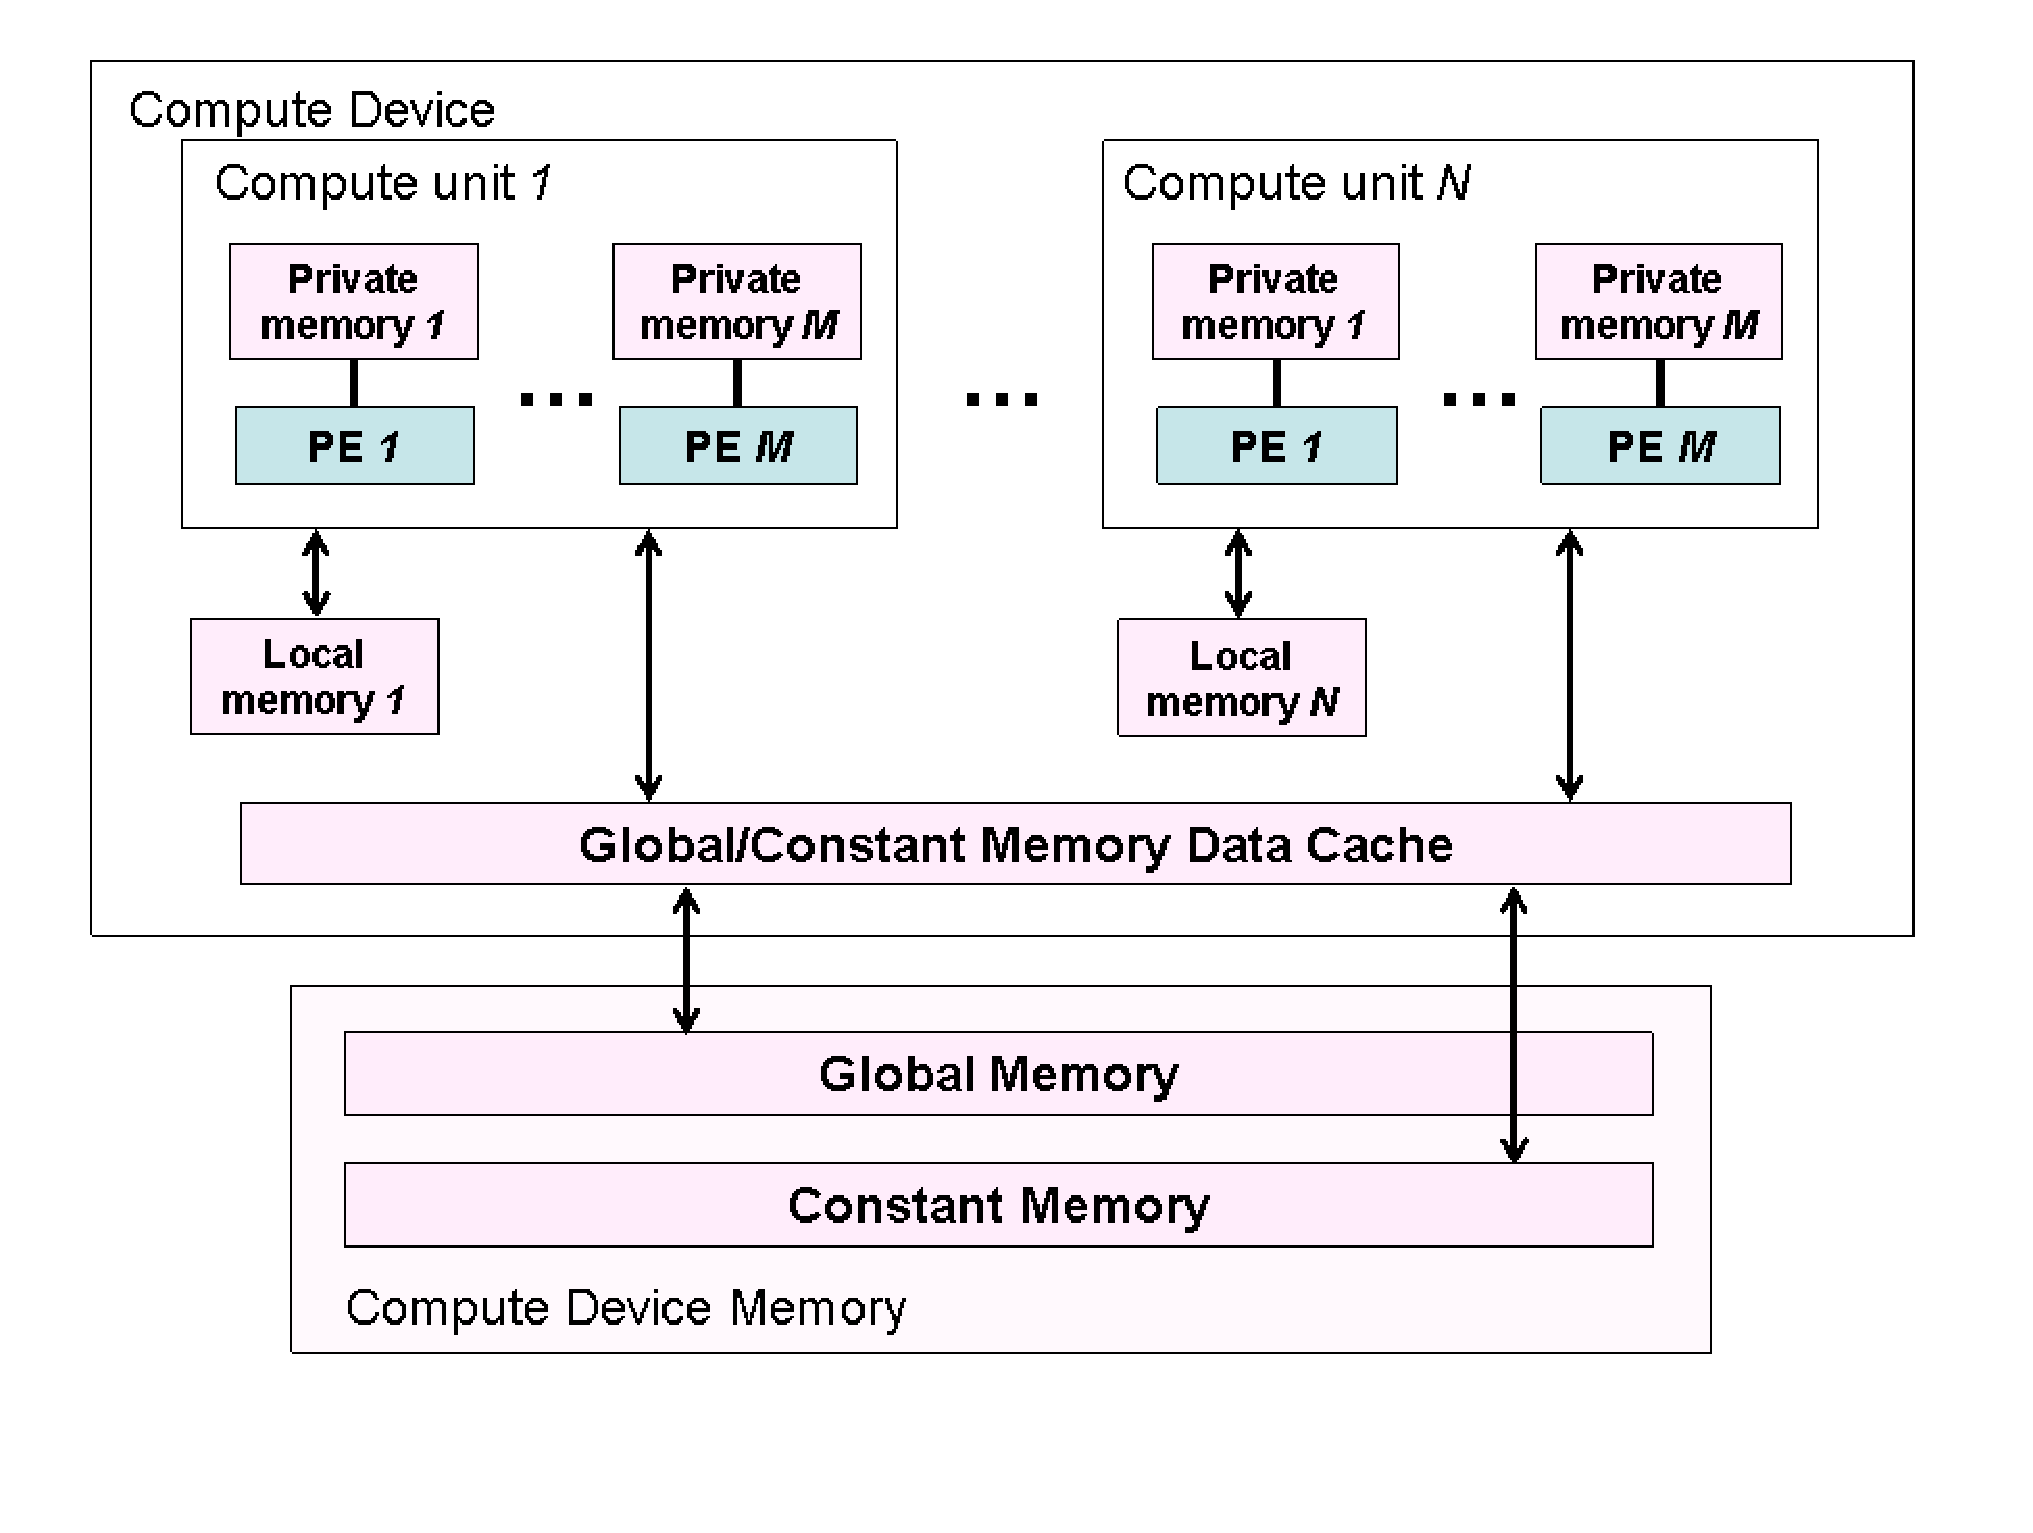
\includegraphics[width=0.95\columnwidth]{kepek/opencl_device.eps}
			\caption{OpenCL ``device'' architektúra \cite{Web:khronos}} 
			\label{fig:device} 
		\end{figure}
		
		A ``compute unit''-ok kiéheztetésének elkerülés végett (több ezer)
		``work-item'' virtuális osztozik rajta.
		Továbbá ezen ``work-item''-ek ``work-group''-okba vannak rendezve, később
		részletezett megfontolások végett.
		A ``compute unit'' kiéhesztetését a ``device''-on található memória chipek lassúsága okozza.
		Ennek hárdveres megoldása a több szintű prediktív cache memória beiktatása a
		``compute unit'' és a külső memória közé.
		Mivel a bank szervezett külső memóriák hozzáférési ideje relatíve nagy
		így a memória szervezésére nagy hangsúlyt kell fektetni.
		
		Az OpenCL négy memória szintet különböztet meg, ami az
		\ref{table:mem} táblázatban és az \ref{fig:device}. ábrán látható.
		Ahhoz, hogy a rendszerben rejlő teljesítményt kihozzuk három fontos kérdést
		kell a szimulátor magjának implementálásakor megválaszolnunk:
		\begin{itemize}
			\item \textbf{Mennyit?}: Tisztában kell lennünk az aktuális
			memória fogyasztással és a szükséges memóriamérettel.
			\item \textbf{Honnan-hova?}: Fontos, hogy a lehető legközelebb legyen az adat
			a ``work-item''-hez.
			\item \textbf{Mikor?}: Mivel a memória művelet alatt a ``work-item'' nem
			dolgozik, így átadja a helyét egy másiknak. Ennek a megfelelő
			szinkronizációjával nagyobb kihasználtság érhető el (load balance).
		\end{itemize}
		
		\begin{table}[!t]
		\renewcommand{\arraystretch}{1.3}
		% if using array.sty, it might be a good idea to tweak the value of
		% \extrarowheight as needed to properly center the text within the cells
		\caption{OpenCL memória szintek}
		\label{table:mem}
		\centering
		% Some packages, such as MDW tools, offer better commands for making tables
		% than the plain LaTeX2e tabular which is used here.
		\resizebox{\columnwidth}{!}{
		\begin{tabular}{l|l|l|l|l}
				 & Global & Constant & Local & Private\\ \hline
			Host & Dinamikusan R/W & Din. R/W & Din. R/W & \\
			Kernel & R/W & Statikusan R & Satik. R/W & Statik. R/W\\
			Sebesség & Lassú & Gyors & Gyors & Regiszter\\
			Méret & $1$ Gbyte $<$ & $\sim64$ Kbyte& $\sim16$ Kbyte & $<1$ Kbyte
		\end{tabular}
		}
		\end{table}
		

		
		OpenCL keretrendszerben történő programozás során két programot kell írnunk.
		Az egyik a ``host''-on fut, ami elvégzi a probléma összeállítását, memória
		allokálását, argumentumok beállítását és a másik program a kernel meghívását a
		``device''-on.
		A kernel futása végeztével a ``host'' program kiolvassa a ``device''-ból
		a kívánt eredményt.
		
	\subsection{Implementációhoz szükséges megfontolások}
		
		A következőkben egy kissebb teljesítményű notebook videókártyát veszek
		alapul a megfontolások demonstrálására. Ez az nVidia GeForce 330M, 
		575 MHz-en futó 48 CUDA core-al, 1024GB memóriával és
		OpenCL 1.0 kompatibilitással.
		A videókártya továbbiakban fontos paraméterei a \ref{table:vcard}. táblázatban
		látható.
		
		\begin{table}[!t]
		\renewcommand{\arraystretch}{1.3}
		% if using array.sty, it might be a good idea to tweak the value of
		% \extrarowheight as needed to properly center the text within the cells
		\caption{nVidia GeForce 330M OpenCL tulajdonságai}
		\label{table:vcard}
		\centering
		% Some packages, such as MDW tools, offer better commands for making tables
		% than the plain LaTeX2e tabular which is used here.
		\begin{tabular}{l|r}
			MAX\_COMPUTE\_UNITS & 6\\
			MAX\_WORK\_GROUP\_SIZES & 512 512 64\\
			GLOBAL\_MEM\_SIZE & 1073020928\\
			MAX\_CONSTANT\_BUFFER\_SIZE & 65536\\
			LOCAL\_MEM\_SIZE & 16384
		\end{tabular}
		\end{table}
		
		
		
		Ha a tér ahol a laplace egyenletet meg kell oldanunk nagyon nagy, akkor
		érdemes szétbontani kissebb alterekre és azokhoz rendelni egy-egy
		``work-item''-eket. Mivel a diszkrét laplace egyenlet egy pontja a szomszédos
		pontokkal szoros kapcsolatban van, így az összefüggő ``work-item"-eket egy
		``work-group''-ba érdemes szervezni, mivel így az átlapolódó pontok értékét a
		szomszédos ``work-item'' is tudják írni és olvasni. Az ilyen típusú
		problémának méretét a MAX\_WORK\_GROUP\_SIZES tulajdonság korlátozza.
		
		Jelen esetben a mérési eredmény egy pontjához tartozó tér átlagosan
		$11\times11\times30$ pontból áll.
		Tehát a korábbi nem áll fenn és egyszerű megfeleltetéssel szétoszthatjuk a
		feladatot.
		A teljes tér $512\times512\times11\times11\times30$ méretű, ami $951k$ pont.
		A tárolásához single-precision mellett ennek a számnak a 4-szerese
		szükségeltetik byte-okban mérva. Mivel ez a videókártyán nem áll
		rendelkezésre, így szétbontjuk kissebb feladatrészekre.
		
		Ezen feladatrészek méretét egy paraméter állításával lehet változtati és az
		implementált algoritmus ettől generikusan függ.
		Emellett az interpoláció mértéke is generikusan paraméterrel állítható.
		Az algoritmus generikusságát csupán a futási időben történő dinamikus memória
		allokációval lehetséges megvalósítani. A korábban említettek végett (\ref{table:mem} táblázat)
		az allokáció csak a ``host'' programban történhet.
	
	\subsection{Memória szervezés}
		\subsubsection{Csak globális memória használata}
		Az algoritmus pszeudó kódjának direkt leképezése esetén a ``host''-on
		allokálunk memóriát a ``device'' globális memóriájában.
		Majd a megfelelő adatokat ide másoljuk és a kernel is itt ír és olvas.
		A problémát a globális memória nagy hozzáférési ideje jelenti, ami miatt sok
		``work-item'' tétlenül a memóriára fog várakozni.
		Ilyenkor az egy mérési pontra vonatkoztatott szimulációs idő a
		referenciánál is lassabb.
		\subsubsection{Globális memória és adott esetben lokális memória használata}
		Kis erőfeszítéssel nagy javulást lehet elérni, ha a mérési ponthoz tartozó
		szimulációs tér éppen belefér a lokális memóriába.
		Tehát, mielött az \ref{eq:2} szerinti iteratív megoldót futtatnánk először a
		globális memóriából a lokális memóriába töltjük át a kérdéses pontokat, majd
		számolunk rajt és a végén visszatöltjük a globális memóriába.
		E javítással a referenciával azonos sebességet tudunk elérni.
		\subsubsection{Globális memória és minden adódó alkalomkor a lokális memória használata}
		Nagyobb erőfeszítést igényel, hogy a globális memórival való kommunikációt a
		lokális memória közbeékelésével tegyünk minden alkalomkor.
		Ezt úgy lehet felfogni, mintha a globális memóriát lokális memória méretű
		kvantumokban tudnám csak elérni.
		Ekkor nagy odafigyelést kíván a memóriacímzés megfelelő prgramozása, de
		eredményképp gyorsulás elérhető. \\
		
		Összegezve elmondható, hogy az aktuálisan használt adat tárolását a lehető
		legközelebb kell tartani a ``compute-unit''-hoz.
	

	
	 \section{Eredmények} 
	\subsection{MATLAB implementációk}
	A referenciaként szolgáló MATLAB algoritmus lineáris programszervezést
	alkalmazva az elérhető fajlagos futási idő $\sim100 ms$.
	
	A kód minimális változtatásával elérhető a párhuzamos végrehajtás. Ezt a
	\texttt{for} ciklusok Parallel Toolbox beli \texttt{parfor} utasítására
	cserélve érhetjük el. 4 processzormaggal rendelkező PC esetén ilyenkor
	közel a negyedére csökken a futási idő.
	
	\subsection{OpenCL implementációk}
	OpenCL keretrendszer segítségével írt programot a GPU-n futtatva a
	\ref{table:openresult} táblázatban látható eredményeket kapjuk.
	Csupán a globális memóriát használva a referenciához képest romlik a
	teljesítmény. Ezt a videókártya prediktív cache nélküli kialakításának és a
	globális memórája okozta kiéheztetésnek tudhatjuk be.
	A lokális memória használata a futási időt drasztikusan le tudja
	csökkenteni, ami a korábban ismertetett memória szervezési gondolatok
	helyességét igazolja.
	 
	\begin{table*}[!t]
	\renewcommand{\arraystretch}{1.2}
	% if using array.sty, it might be a good idea to tweak the value of
	% \extrarowheight as needed to properly center the text within the cells
	\caption{\scriptsize OpenCL futási idő eredmények $12\times12$ mérési pontra}
	\label{table:openresult}
	% Some packages, such as MDW tools, offer better commands for making tables
	% than the plain LaTeX2e tabular which is used here.
	\centering
	\begin{tabular}{l|r|r|r}
	 & Globális memória & Lokális memória, ha befér & Lokális memória bufferelés\\ \hline
	\parbox{2.5cm}{Globális tranzakciók száma átlagosan} & $12 \times 12\times 32.3$
	& $12 \times 12 \times 32.3$ & $12 \times 12 \times 32.3$\\
	\parbox{2.5cm}{Lokális tranzakciók száma átlagosan} & 0 &
	$0.48 \times 12 \times 12 \times 30$ & $2.08 \times 12 \times12 \times 32.3$\\
	Futási idő & 5990 ms & 2530 ms & 510 ms\\
	Fajlagos futási idő & 410 ms & 170 ms & 3.5 ms 
	\end{tabular}
	\end{table*}
	
	\begin{figure*}[!t]
		\centering
		\subfloat[Mérési eredmény]{\includegraphics[width=0.45\columnwidth]{kepek/eps/afm200.eps}%
		\label{fig_first_case}}
		\hfil
		\subfloat[Szimulációs eredmény]{\includegraphics[width=0.45\columnwidth]{kepek/eps/efm200.eps}%
		\label{fig_second_case}}
		\caption{\scriptsize Méréssel kapott felület (balra) és szimulációval kapott töltéstérkép}
		\label{fig_sim}
	\end{figure*}
	

	
	\section{Összegzés}
A cikkünkben ismertettük az AFM mérések validálásának problémáját.
A szimulálandó problémát ismertetve adódott a párhuzamosítás lehetősége.
A hordozhatóság és a gyorsabb végrehajtás végett a szimulátort OpenCL
környezetben implementáltuk.
Ismertettük az implementáció során észben tartandó gondolatokat, azok
általánosságának elvesztése nélkül.

Az eredményeket ismertetve látványos gyorsulást tapasztaltunk, ami nehezebben
kezelhető problémáknál azonos futási idő mellett nagyob pontosságot jelenthet.  



	
	
	\bibliography{mybib.bib}
%	\addcontentsline{toc}{chapter}{Irodalomjegyzék}
	\bibliographystyle{IEEEtran}
	
	%\begin{thebibliography}{1}
	
	%\bibitem{Web:khronos}
	%The Khronos OpenCL Working Group, \emph{“OpenCL - The open stan-
	%dard for parallel programming of heterogeneous systems.”} \\http://www.
	%khronos.org/opencl/, 2014.
	%\end{thebibliography}
	
\end{document}
